% =====================================================================
%  CricketMind -- Architecture Draft v2
%  A Multi-Modal Multi-Agent System for Cricket Analytics
%
%  Revision notes vs. v1:
%    * Expands the worker layer from 6 unnamed workers to the full
%      14-agent roster: 12 stakeholder-facing agents + 2 shared
%      analytical services.
%    * Fills the N9/N10/N11 numbering gap left blank in the v1 figure.
%    * Separates "analytical services" (N8, N9) from "stakeholder
%      agents" (N11a-N11l), which is the key structural change.
%
%  Compile with: pdflatex CricketMind_Architecture_v2.tex   (run twice)
% =====================================================================
\documentclass[11pt,a4paper]{article}

\usepackage[margin=2cm]{geometry}
\usepackage[T1]{fontenc}
\usepackage[utf8]{inputenc}
\usepackage{lmodern}
\usepackage{booktabs}
\usepackage{array}
\usepackage{xcolor}
\usepackage{amsmath}
\usepackage{enumitem}
\usepackage{float}
\usepackage{capt-of}
\usepackage{tikz}
\usetikzlibrary{shapes.geometric,arrows.meta,positioning,calc,fit,backgrounds}
\usepackage[hidelinks]{hyperref}

% ---------------------------------------------------------------- colours
\definecolor{encblue}{RGB}{31,58,110}      % vision / text encoding
\definecolor{fuseteal}{RGB}{17,110,110}    % multimodal fusion
\definecolor{retbrown}{RGB}{124,76,38}     % retrieval
\definecolor{svcorange}{RGB}{176,90,20}    % shared analytical services
\definecolor{routeviolet}{RGB}{88,48,132}  % supervisor / router
\definecolor{agentgreen}{RGB}{27,94,58}    % stakeholder agents
\definecolor{gatered}{RGB}{170,30,40}      % confidence gate
\definecolor{gatepurple}{RGB}{112,44,132}  % faithfulness gate
\definecolor{dbtan}{RGB}{222,196,160}      % databases
\definecolor{outgrey}{RGB}{45,45,50}       % final output
\definecolor{gateslate}{RGB}{72,88,104}    % entry branch

% ---------------------------------------------------------------- styles
\tikzset{
  base/.style   = {draw, rounded corners=2pt, align=center, font=\small,
                   text width=2.9cm, minimum height=1.1cm, inner sep=3pt,
                   line width=0.7pt},
  enc/.style    = {base, fill=encblue,     text=white, draw=encblue!55!black},
  fuse/.style   = {base, fill=fuseteal,    text=white, draw=fuseteal!55!black},
  ret/.style    = {base, fill=retbrown,    text=white, draw=retbrown!55!black},
  svc/.style    = {base, fill=svcorange,   text=white, draw=svcorange!55!black},
  route/.style  = {base, fill=routeviolet, text=white, draw=routeviolet!55!black},
  agent/.style  = {base, fill=agentgreen,  text=white, draw=agentgreen!55!black,
                   text width=2.7cm, minimum height=1.2cm, font=\footnotesize},
  outnode/.style    = {base, fill=outgrey,     text=white, draw=black},
  gate/.style   = {draw, diamond, aspect=2.0, align=center,
                   font=\footnotesize\bfseries, inner sep=2pt, line width=0.7pt},
  confgate/.style  = {gate, fill=gatered,    text=white, draw=gatered!55!black},
  faithgate/.style = {gate, fill=gatepurple, text=white, draw=gatepurple!55!black},
  entrygate/.style = {gate, fill=gateslate,  text=white, draw=gateslate!55!black},
  db/.style     = {draw, cylinder, shape border rotate=90, aspect=0.28,
                   fill=dbtan, align=center, font=\scriptsize,
                   minimum width=1.8cm, minimum height=1.0cm, line width=0.7pt},
  flow/.style   = {-{Stealth[length=2.4mm]}, line width=0.9pt, draw=black!72},
  bus/.style    = {line width=0.9pt, draw=black!72},
  redloop/.style   = {-{Stealth[length=2.4mm]}, line width=0.9pt,
                   draw=gatered, dashed, dash pattern=on 4pt off 2.5pt},
  yield/.style  = {-{Stealth[length=2.2mm]}, line width=0.8pt,
                   draw=agentgreen!85, dashed, dash pattern=on 3pt off 2pt},
  ybus/.style   = {line width=0.8pt, draw=agentgreen!85, dashed,
                   dash pattern=on 3pt off 2pt},
  elab/.style   = {font=\scriptsize\itshape, inner sep=1.5pt, fill=white},
}

\title{\textbf{CricketMind}\\[0.3em]
       \large A Multi-Modal Multi-Agent System for Cricket Analytics\\[0.2em]
       \normalsize Thesis Architecture Draft --- Version 2 (14-Agent Roster)}
\author{}
\date{}

\begin{document}
\maketitle
\thispagestyle{empty}

% =====================================================================
\section{The Core Concept}

\subsection*{The Problem}
Modern cricket analytics is heavily siloed. Visual analysis (a coach reviewing
batting technique on video) and statistical analysis (an analyst studying strike
rates and match-ups) are performed completely independently. No existing
artificial intelligence system automatically bridges the gap between what a
cricket shot \emph{looks like} (kinematics) and what its historical outcome
\emph{is} (statistics). Furthermore, attempting to solve complex sports queries
with a single Large Language Model (LLM) results in hallucination and loss of
reasoning context.

A second, subtler problem motivates this revision. Cricket is not consumed by a
single kind of user. A franchise director, a bowling coach, a physiotherapist and
a broadcast producer all need answers derived from the \emph{same} underlying
delivery, but expressed in entirely different vocabularies, at different time
horizons, and under different constraints. A monolithic ``analytics assistant''
collapses these into one averaged voice that serves none of them well.

\subsection*{The Solution: CricketMind}
\textbf{CricketMind} is a multi-modal, multi-agent system (MAS) built on the
LangGraph framework. Rather than relying on a single AI brain, the system
delegates analytical work to a decentralised \emph{team} of specialised agents,
coordinated by a supervisor.

The system takes two inputs simultaneously:
\begin{enumerate}[nosep,leftmargin=1.6em]
  \item A natural-language query, e.g.\ \emph{``What is the tactical weakness of
        this batsman against spin?''}
  \item A raw video clip of the batsman in action.
\end{enumerate}

% =====================================================================
\clearpage
\section{System Architecture Diagram}

% ---------------------------------------------------------------------
%  NOT a float.  A float this large cannot be placed by LaTeX and is
%  silently dropped (which is exactly what happened in v2.0: section 2
%  rendered as a heading with nothing under it).  A plain centred box
%  cannot be lost.  Layout is deliberately wide-and-short so the whole
%  picture fits one portrait page after scaling to \textwidth.
% ---------------------------------------------------------------------
\begin{center}
\resizebox{\textwidth}{!}{%
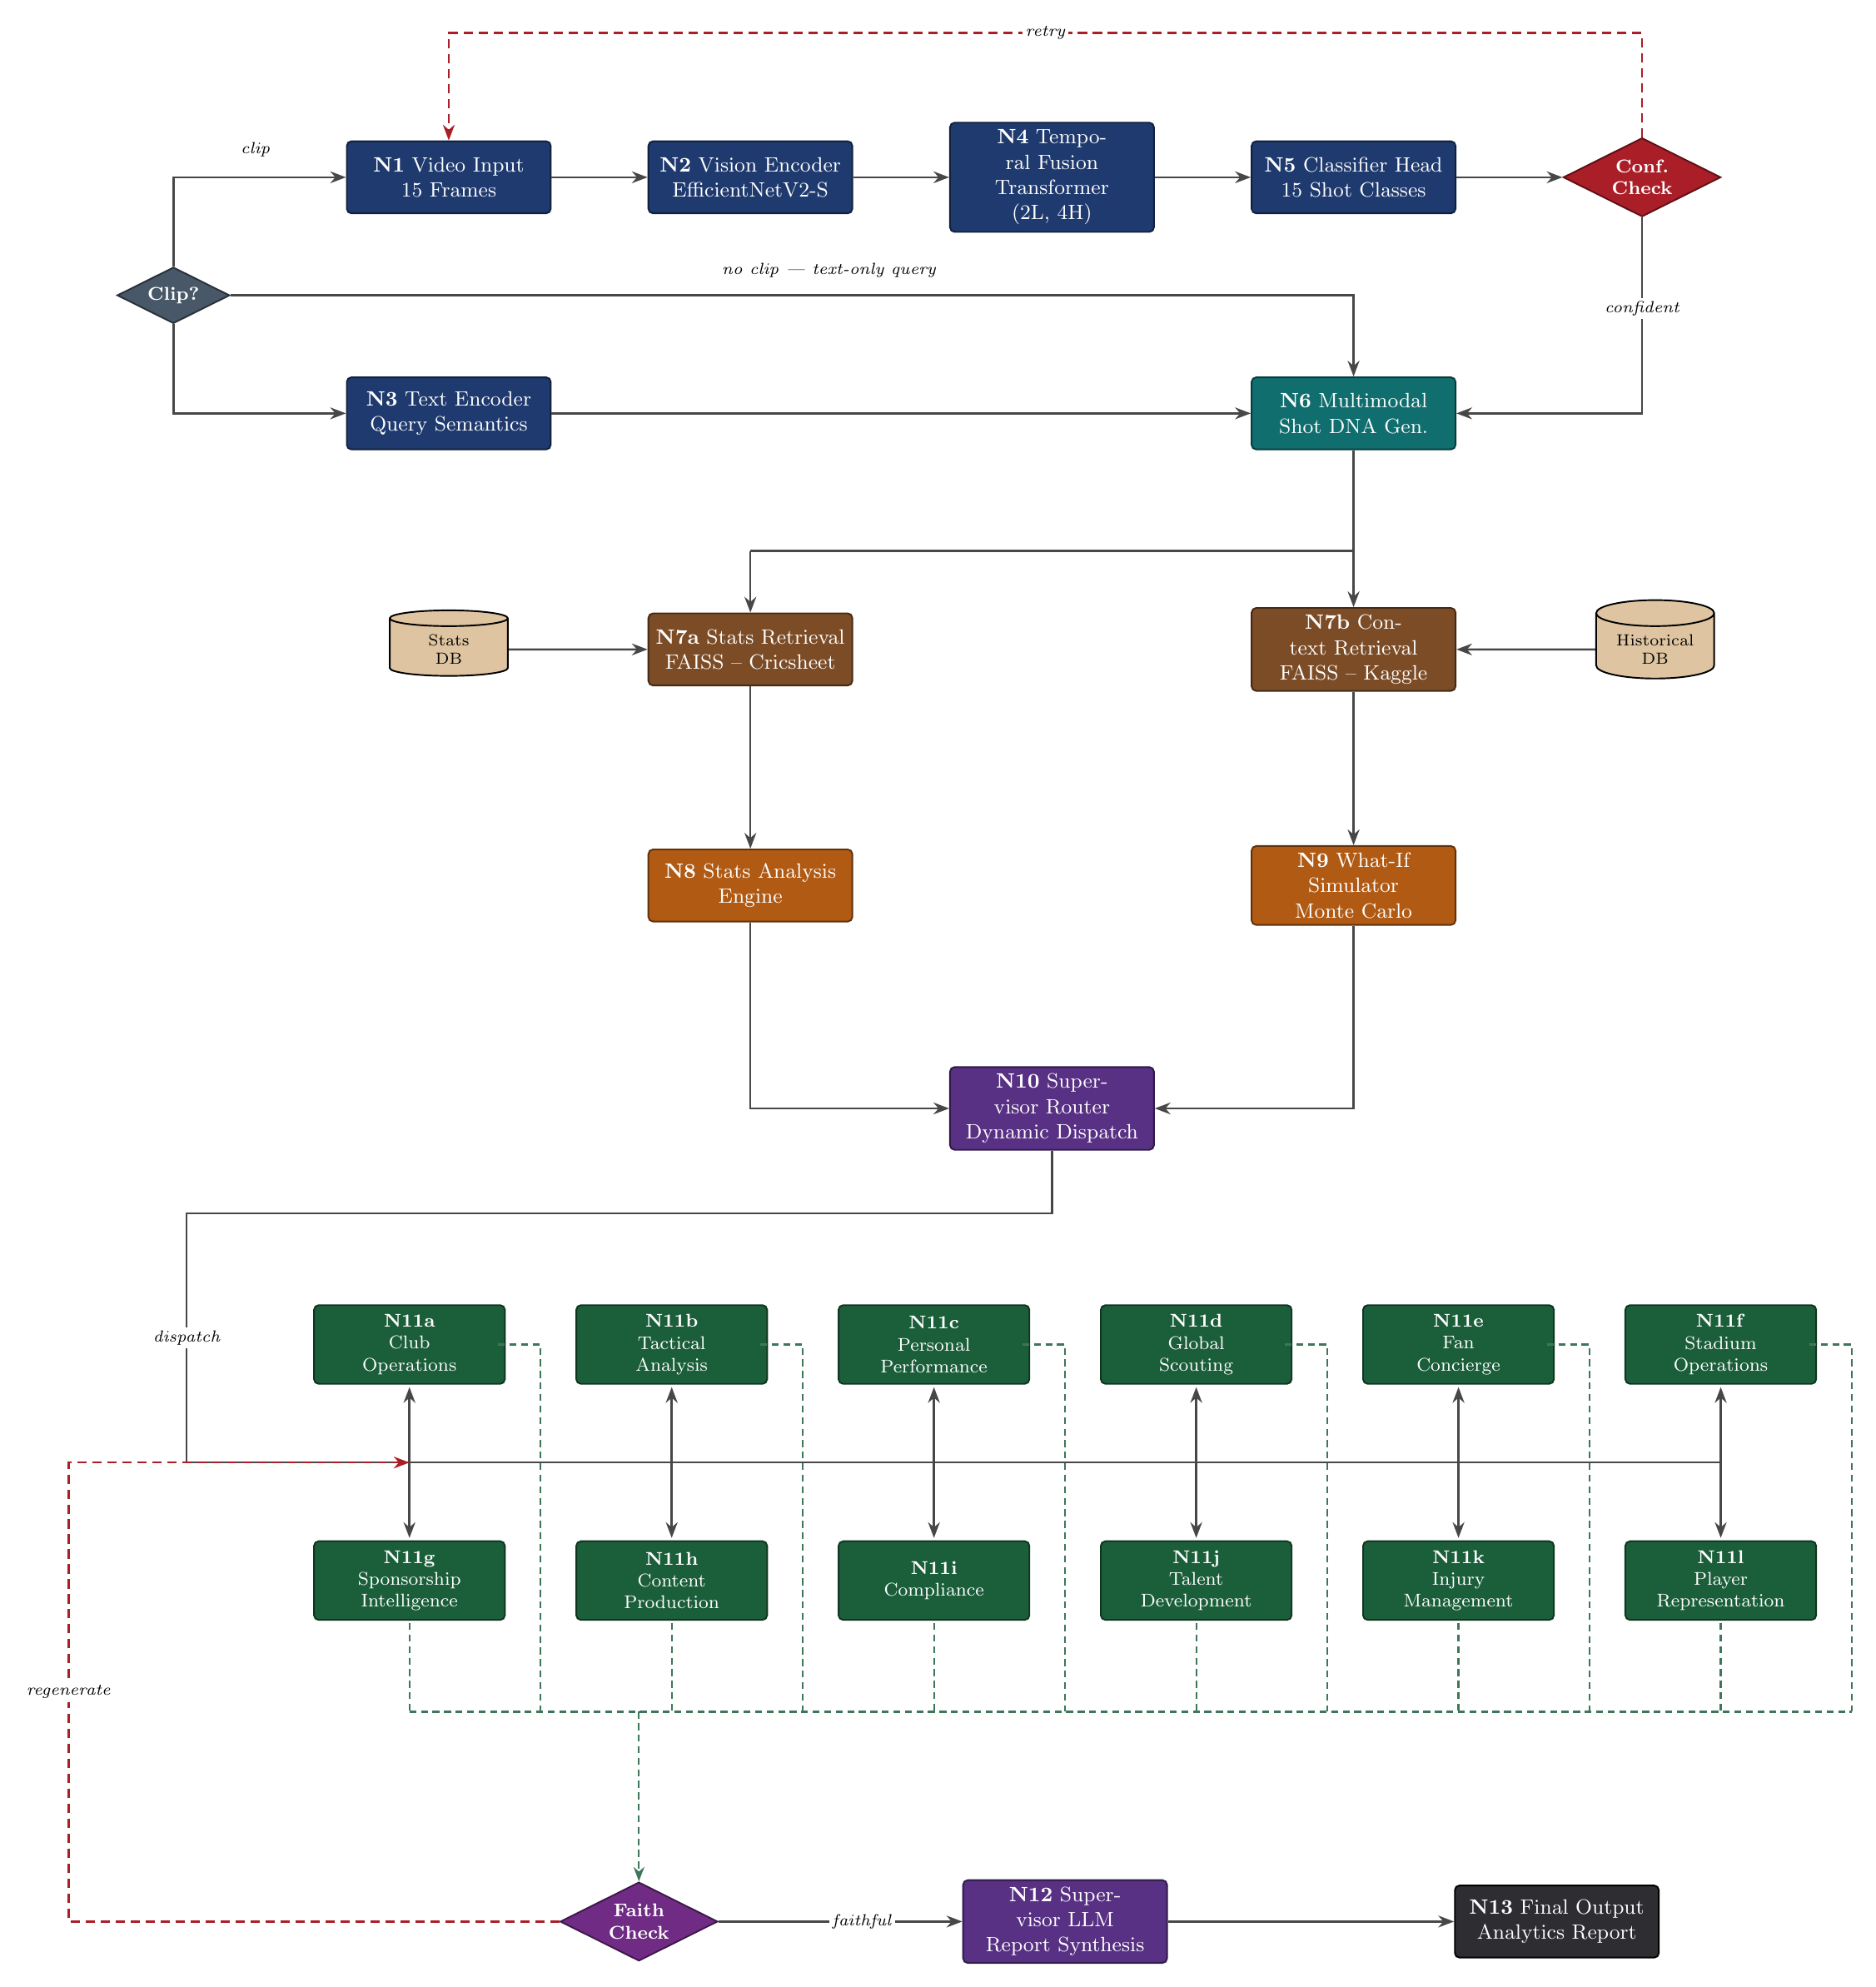
\begin{tikzpicture}

% ============================================ 0. entry branch
% Not every query carries a clip.  A counterfactual about batting order has
% no video, so the vision chain must be skippable.
\node[entrygate] (entry) at (-2.6,-1.8) {Clip?};

% ============================================ A. encoding chain (horizontal)
\node[enc] (n1)   at (1.6,0)    {\textbf{N1} Video Input\\15 Frames};
\node[enc] (n2)   at (6.2,0)    {\textbf{N2} Vision Encoder\\EfficientNetV2-S};
\node[enc] (n4)   at (10.8,0)   {\textbf{N4} Temporal Fusion\\Transformer (2L, 4H)};
\node[enc] (n5)   at (15.4,0)   {\textbf{N5} Classifier Head\\15 Shot Classes};
\node[confgate] (conf) at (19.8,0) {Conf.\\Check};

% ============================================ B. text branch + grounding
\node[enc]  (n3) at (1.6,-3.6)  {\textbf{N3} Text Encoder\\Query Semantics};
\node[fuse] (n6) at (15.4,-3.6) {\textbf{N6} Multimodal\\Shot DNA Gen.};

% ============================================ C. retrieval
\node[db]  (db1) at (1.6,-7.2)  {Stats\\DB};
\node[ret] (n7a) at (6.2,-7.2)  {\textbf{N7a} Stats Retrieval\\FAISS -- Cricsheet};
\node[ret] (n7b) at (15.4,-7.2) {\textbf{N7b} Context Retrieval\\FAISS -- Kaggle};
\node[db]  (db2) at (20.0,-7.2) {Historical\\DB};

% ============================================ D. shared analytical services
\node[svc] (n8) at (6.2,-10.8)  {\textbf{N8} Stats Analysis\\Engine};
\node[svc] (n9) at (15.4,-10.8) {\textbf{N9} What-If Simulator\\Monte Carlo};

% ============================================ E. supervisor router
\node[route] (n10) at (10.8,-14.2) {\textbf{N10} Supervisor Router\\Dynamic Dispatch};

% ============================================ F. twelve stakeholder agents
% Written out explicitly rather than with \foreach: a "\\" inside a
% \foreach value list is a known pgffor failure point.
\node[agent] (ag1)  at (1,-17.8)  {\textbf{N11a}\\Club\\Operations};
\node[agent] (ag2)  at (5,-17.8)  {\textbf{N11b}\\Tactical\\Analysis};
\node[agent] (ag3)  at (9,-17.8)  {\textbf{N11c}\\Personal\\Performance};
\node[agent] (ag4)  at (13,-17.8) {\textbf{N11d}\\Global\\Scouting};
\node[agent] (ag5)  at (17,-17.8) {\textbf{N11e}\\Fan\\Concierge};
\node[agent] (ag6)  at (21,-17.8) {\textbf{N11f}\\Stadium\\Operations};

\node[agent] (ag7)  at (1,-21.4)  {\textbf{N11g}\\Sponsorship\\Intelligence};
\node[agent] (ag8)  at (5,-21.4)  {\textbf{N11h}\\Content\\Production};
\node[agent] (ag9)  at (9,-21.4)  {\textbf{N11i}\\Compliance};
\node[agent] (ag10) at (13,-21.4) {\textbf{N11j}\\Talent\\Development};
\node[agent] (ag11) at (17,-21.4) {\textbf{N11k}\\Injury\\Management};
\node[agent] (ag12) at (21,-21.4) {\textbf{N11l}\\Player\\Representation};

% ============================================ G. synthesis (horizontal)
\node[faithgate] (faith) at (4.5,-26.6) {Faith\\Check};
\node[route] (n12) at (11,-26.6)   {\textbf{N12} Supervisor LLM\\Report Synthesis};
\node[outnode]   (n13) at (18.5,-26.6) {\textbf{N13} Final Output\\Analytics Report};

% ==================================================================
%                              EDGES
% ==================================================================

% ---- entry branch.  The bypass runs in the clear lane at y=-1.8: below the
%      encoder row, above the text row, and left of the confident edge at
%      x=19.8.  It enters N6 from the north so it misses the N3 -> N6 run.
\draw[flow] (entry.north) -- (-2.6,0) -- (n1.west);
\node[elab] at (-1.35,0.42) {clip};
\draw[flow] (entry.south) -- (-2.6,-3.6) -- (n3.west);
\draw[flow] (entry.east)  -- (15.4,-1.8) -- (n6.north);
\node[elab] at (7.4,-1.42) {no clip --- text-only query};

% ---- encoding chain
\draw[flow] (n1) -- (n2);
\draw[flow] (n2) -- (n4);
\draw[flow] (n4) -- (n5);
\draw[flow] (n5) -- (conf);

% ---- retry loop: runs above the chain, clear of every node
\draw[redloop] (conf.north) -- (19.8,2.2) -- (1.6,2.2) -- (n1.north);
\node[elab] at (10.7,2.2) {retry};

% ---- confident -> Shot DNA
\draw[flow] (conf.south) -- (19.8,-3.6) -- (n6.east);
\node[elab] at (19.8,-2.0) {confident};

% ---- text encoder -> Shot DNA (straight horizontal run)
\draw[flow] (n3.east) -- (n6.west);

% ---- Shot DNA -> both retrievers
\draw[bus]  (n6.south) -- (15.4,-5.7);
\draw[bus]  (6.2,-5.7) -- (15.4,-5.7);
\draw[flow] (6.2,-5.7)  -- (n7a.north);
\draw[flow] (15.4,-5.7) -- (n7b.north);

% ---- databases -> retrievers
\draw[flow] (db1) -- (n7a);
\draw[flow] (db2) -- (n7b);

% ---- retrievers -> analytical services
\draw[flow] (n7a) -- (n8);
\draw[flow] (n7b) -- (n9);

% ---- analytical services -> router
\draw[flow] (n8.south) -- (6.2,-14.2)  -- (n10.west);
\draw[flow] (n9.south) -- (15.4,-14.2) -- (n10.east);

% ---- router -> dispatch bus, routed around the left edge so it does not
%      collide with the row-1 output gutters
\draw[bus] (n10.south) -- (10.8,-15.8) -- (-2.4,-15.8) -- (-2.4,-19.6) -- (1,-19.6);
\draw[bus] (1,-19.6) -- (21,-19.6);
\node[elab] at (-2.4,-17.7) {dispatch};

% ---- dispatch bus -> each agent (up into row 1, down into row 2)
\draw[flow] (1,-19.6)  -- (1,-18.45);
\draw[flow] (5,-19.6)  -- (5,-18.45);
\draw[flow] (9,-19.6)  -- (9,-18.45);
\draw[flow] (13,-19.6) -- (13,-18.45);
\draw[flow] (17,-19.6) -- (17,-18.45);
\draw[flow] (21,-19.6) -- (21,-18.45);

\draw[flow] (1,-19.6)  -- (1,-20.75);
\draw[flow] (5,-19.6)  -- (5,-20.75);
\draw[flow] (9,-19.6)  -- (9,-20.75);
\draw[flow] (13,-19.6) -- (13,-20.75);
\draw[flow] (17,-19.6) -- (17,-20.75);
\draw[flow] (21,-19.6) -- (21,-20.75);

% ---- collection bus (green dashed) below row 2
\draw[ybus] (1,-23.4) -- (23,-23.4);

% row 2 drops straight down
\draw[ybus] (1,-22.05)  -- (1,-23.4);
\draw[ybus] (5,-22.05)  -- (5,-23.4);
\draw[ybus] (9,-22.05)  -- (9,-23.4);
\draw[ybus] (13,-22.05) -- (13,-23.4);
\draw[ybus] (17,-22.05) -- (17,-23.4);
\draw[ybus] (21,-22.05) -- (21,-23.4);

% row 1 exits east and drops through the gutter between columns
\draw[ybus] (2.35,-17.8)  -- (3,-17.8)  -- (3,-23.4);
\draw[ybus] (6.35,-17.8)  -- (7,-17.8)  -- (7,-23.4);
\draw[ybus] (10.35,-17.8) -- (11,-17.8) -- (11,-23.4);
\draw[ybus] (14.35,-17.8) -- (15,-17.8) -- (15,-23.4);
\draw[ybus] (18.35,-17.8) -- (19,-17.8) -- (19,-23.4);
\draw[ybus] (22.35,-17.8) -- (23,-17.8) -- (23,-23.4);

% ---- collection bus -> faith check
\draw[yield] (4.5,-23.4) -- (faith.north);

% ---- faith check -> synthesis -> output
\draw[flow] (faith.east) -- (n12.west);
\node[elab] at (7.9,-26.6) {faithful};
\draw[flow] (n12.east) -- (n13.west);

% ---- regenerate loop: back to the dispatch bus
\draw[redloop] (faith.west) -- (-4.2,-26.6) -- (-4.2,-19.6) -- (1,-19.6);
\node[elab] at (-4.2,-23.1) {regenerate};

\end{tikzpicture}}

\captionof{figure}{Full CricketMind LangGraph architecture (Version~2). Blue
nodes perform visual and textual encoding; the teal node fuses both modalities
into the Shot DNA record; brown nodes retrieve grounding evidence from the two
FAISS indexes; orange nodes are the two shared analytical services that hold
exclusive authority to emit numeric claims; green nodes are the twelve
stakeholder-facing agents dispatched dynamically by the violet supervisor
router. Red diamonds and red dashed edges are the two agentic correction loops;
green dashed edges carry agent findings back to the faithfulness gate. The slate
diamond at the left is the entry branch: only a query carrying a clip enters the
vision chain, while a text-only question --- a counterfactual about batting
order, for instance --- passes directly to N6 and is grounded on its query
filters alone. N3 runs on both paths, because every query has text.}
\label{fig:arch-v2}
\end{center}

% =====================================================================
\clearpage
\section{Node-by-Node Explanation}

To make the flow concrete we trace a single user query end to end.

\begin{quote}
\textbf{Running Example.} \emph{``Compare Virat Kohli's Cover Drive vs.\ his Pull
Shot against fast bowlers in the powerplay.''}
\end{quote}

% ------------------------------------------------------------------
\subsection{Two Entry Paths}

Not every question carries a clip. \emph{``What if Rohit Sharma had batted at
number two instead of Kohli?''} is a legitimate query with no video attached:
there is no stroke to classify, and nothing for the confidence gate to
adjudicate. The graph therefore branches at entry.

A query carrying a clip enters the vision chain at N1 and reaches N6 through the
confidence gate, exactly as described below. A text-only query bypasses
N1--N5 entirely and arrives at N6 directly, where it is grounded on the filters
N3 extracted from its own text. N3 runs on both paths, because every query has
text.

The consequence propagates further than the diagram suggests. On the text-only
path no posture was ever measured, so \texttt{weight\_transfer} is \emph{absent}
from the sanctioned facts rather than defaulted. Supplying a default would place
an invented measurement into the exact surface the faithfulness gate treats as
ground truth --- a fabrication laundered through the mechanism designed to stop
fabrications. The supervisor router reads the same rule and declines to wake any
agent whose citations cannot be satisfied, which on this path removes the
Personal Performance (N11c) and Talent Development (N11j) agents. The resulting
report is shorter, and everything remaining in it is still grounded.

% ------------------------------------------------------------------
\subsection{Vision and Text Processing Layer (Blue Nodes)}

\begin{description}[leftmargin=0em,style=nextline]
\item[N1 --- Video Input (15 Frames).]
  Reached only when the query carries a clip. The user uploads footage of Kohli
  batting, and the system uniformly samples
  \textbf{15 frames}, which is the temporal resolution the downstream backbone
  was trained on. Fifteen frames at roughly one second of footage is enough to
  capture the full stroke arc --- backlift, stride, contact, follow-through ---
  without paying for redundant near-duplicate frames.

\item[N2 --- Vision Encoder (EfficientNetV2-S).]
  Each of the 15 frames is passed through an EfficientNetV2-S backbone,
  producing a per-frame spatial embedding that encodes bat position, body
  posture, foot placement and ball location. The encoder is applied
  frame-independently; no temporal reasoning happens here.

\item[N3 --- Text Encoder (Query Semantics).]
  The natural-language query is embedded so that the system understands it must
  restrict attention to \emph{fast bowlers} and the \emph{powerplay}. Critically,
  N3 runs \textbf{in parallel} with the vision branch --- it does not wait for
  classification --- because its output is needed to parameterise retrieval, not
  to influence what the video contains.

\item[N4 --- Temporal Fusion (Temporal Transformer).]
  A lightweight transformer encoder --- two layers, four attention heads,
  learnable positional embeddings and temporal mean pooling --- consumes the
  ordered sequence of per-frame embeddings and models the stroke as a whole.
  Self-attention is precisely why this stage is not recurrent. In a gated
  recurrent unit, information from the pre-delivery stance reaches the
  follow-through only by surviving every intervening hidden state; under
  self-attention the first and last frames are a single attention hop apart.
  That direct long-range coupling is what separates strokes which differ not in
  their individual frames but in the ordering and velocity profile of the swing
  --- the sweep and the reverse sweep being the canonical confusion pair for the
  recurrent baseline this replaces.

\item[N5 --- Classifier Head (15 Shot Classes).]
  A linear head projects the fused temporal representation onto the 15
  CricShot10k shot classes and produces a probability distribution.
  \emph{Example output:} $92\%$ probability of \textbf{Cover Drive}.
\end{description}

% ------------------------------------------------------------------
\subsection{Validation and Grounding (Red Diamond, Teal Node)}

\begin{description}[leftmargin=0em,style=nextline]
\item[Confidence Check (Red Diamond).]
  If the top-1 classifier probability falls below a set threshold (e.g.\ $70\%$),
  the red dashed \emph{retry} loop is triggered: the system re-enters N1 and
  attempts recovery by requesting an alternate camera angle, re-sampling a
  different 16-frame window, or applying test-time augmentation. The loop is
  bounded by a maximum retry count; on exhaustion the system degrades gracefully
  and reports low visual confidence rather than fabricating a label. This gate
  exists because \emph{every} downstream claim is conditioned on the shot label
  --- an incorrect label silently poisons all fourteen agents.

\item[N6 --- Multimodal Shot DNA Generation.]
  The accepted classification is fused with the query embedding from N3 and with
  continuous visual posture metrics (weight transfer, bat-face angle, stride
  length) into a single structured record we call the \textbf{Shot DNA}. This
  record is the sole interface between the perception half of the system and the
  analytics half: everything after N6 consumes Shot DNA and never touches raw
  pixels again.

  N6 is also the entry point for text-only queries, where there is no
  classification and no posture to fuse. The Shot DNA then carries the query
  filters alone and records which modality produced it, so that every downstream
  node --- and the sanctioned-fact surface in particular --- can tell a measured
  value from an absent one.
\end{description}

% ------------------------------------------------------------------
\subsection{Retrieval Layer (Brown Nodes)}

\begin{description}[leftmargin=0em,style=nextline]
\item[N7a --- Stats Retrieval (FAISS, Cricsheet).]
  Queries the ball-by-ball index for the precise conjunction implied by the Shot
  DNA and the query: \emph{Kohli $+$ Cover Drive $+$ Powerplay $+$ Pace}. This
  returns the narrow, high-precision evidence set.

\item[N7b --- Context Retrieval (FAISS, Kaggle).]
  Retrieves the broader historical envelope --- Kohli's overall strike rate at
  this venue, his career trend against pace, comparable players. This is the
  low-precision, high-recall evidence set that prevents the system from
  over-fitting its narrative to a handful of deliveries.
\end{description}

% ------------------------------------------------------------------
\subsection{Shared Analytical Services (Orange Nodes)}

These two nodes are new in Version~2. They are not stakeholder agents; they have
no audience of their own. They are \textbf{computational engines} that convert
retrieved evidence into verified quantities, and they hold exclusive authority to
emit a number. Every agent in the tier above consumes their output rather than
performing arithmetic inside its own prompt.

\begin{description}[leftmargin=0em,style=nextline]
\item[N8 --- Statistical Analysis Engine.]
  Performs the deterministic aggregation over the retrieved ball-by-ball records:
  strike rates, dismissal frequencies, control percentages, match-up splits.
  \emph{Example output:} Kohli's strike rate is \textbf{142} on cover drives but
  only \textbf{112} on pull shots within the powerplay. Because this node is
  ordinary computation rather than generation, its results are reproducible and
  independently checkable --- which is precisely what makes the faithfulness gate
  downstream meaningful.

\item[N9 --- What-If Simulator (Monte Carlo).]
  Answers counterfactual questions that no historical record can answer directly,
  by sampling forward from the retrieved distributions.
  \emph{Example:} \emph{``What if the bowler sends down six consecutive
  back-of-a-length deliveries?''} The Monte Carlo simulation returns a
  \textbf{40\% chance} of Kohli being dismissed attempting the pull. This node is
  the system's only source of forward-looking, non-observational claims, and its
  outputs are always emitted with explicit uncertainty bounds.
\end{description}

% ------------------------------------------------------------------
\subsection{Supervisor Router (Violet Node)}

\begin{description}[leftmargin=0em,style=nextline]
\item[N10 --- Supervisor Router (Dynamic Dispatch).]
  Inspects the Shot DNA, the query embedding and the analytical results, then
  activates \textbf{only the relevant subset} of the twelve stakeholder agents.
  A technique question wakes the Personal Performance and Talent Development
  agents; an in-match tactical question wakes Tactical Analysis; a workload
  question wakes Injury Management. Dispatching all twelve on every query would
  be both wasteful and harmful --- it would bury the answer in irrelevant
  perspectives. Routing is the mechanism by which a 14-agent system stays
  legible.
\end{description}

% ------------------------------------------------------------------
\subsection{The Twelve Stakeholder Agents (Green Nodes)}

Each agent owns one stakeholder. It shares the same evidence as every other agent
but differs in vocabulary, time horizon and output format.

\begin{description}[leftmargin=0em,style=nextline]
\item[N11a --- Club Operations Agent (Franchises / Boards).]
  Squad budget modelling, IPL/BBL auction simulation, fixture scheduling, staff
  workflow coordination, travel logistics, contract-expiry alerts.

\item[N11b --- Tactical Analysis Agent (Coaches).]
  Ball-by-ball opposition profiling, pitch-condition-aware field placement,
  bowling strategy by match-up, batting order simulation, match scenario
  planning. On the running example this agent recommends bowling short to Kohli,
  reading directly off the pull-shot deficit computed by N8.

\item[N11c --- Personal Performance Agent (Players).]
  Shot-selection trend analysis, format-specific technique profiling, training
  load personalisation, milestone tracking, mental readiness integration. Here it
  notes that Kohli's visual weight transfer on the cover drive is excellent,
  reading the posture metrics carried in the Shot DNA.

\item[N11d --- Global Scouting Agent (Scouts).]
  Aggregates domestic and T20 league metrics across 20$+$ leagues, identifies
  emerging markets (Nepal, UAE, Afghanistan, USA), contract-cycle tracking,
  skill-gap-versus-franchise filtering.

\item[N11e --- Fan Concierge Agent (Fans).]
  Personalised highlight reels, live commentary preference engine, stadium
  wayfinding, ticket booking assistance, fantasy cricket advisory, merchandise
  recommendations.

\item[N11f --- Stadium Operations Agent (Stadiums).]
  Pitch curatorship with moisture and grass sensor integration, crowd flow
  modelling, concession demand forecasting, DRS review room scheduling, floodlight
  energy management.

\item[N11g --- Sponsorship Intelligence Agent (Sponsors).]
  Broadcast jersey and logo visibility scoring, audience demographic indexing,
  social media impression ROI, multilingual reach analysis, proposal
  auto-drafting.

\item[N11h --- Content Production Agent (Broadcasters).]
  Auto-generates multilingual commentary (Hindi, Bengali, Tamil, Sinhala,
  English), pitch map and wagon wheel overlays, highlights clipping, statistical
  ticker automation.

\item[N11i --- Compliance Agent (Governing Bodies).]
  ICC window conflict detection, player eligibility checks, franchise financial
  auditing, ACSU flag aggregation, bio-bubble protocol monitoring.

\item[N11j --- Talent Development Agent (Academies).]
  Personalised skill-acquisition roadmaps, age-group benchmark comparison
  (U-16 $\rightarrow$ U-19 $\rightarrow$ senior), drill recommendation, physical
  literacy progression tracking.

\item[N11k --- Injury Management Agent (Medical Teams).]
  Bowling workload tracking against overs-per-week thresholds, soft-tissue risk
  prediction, return-to-play timelines, session load versus fatigue modelling,
  hamstring and stress fracture flagging.

\item[N11l --- Player Representation Agent (Player Agents / Managers).]
  IPL auction valuation modelling, overseas league slot gap analysis, franchise
  squad roster scanning, market-demand heat maps by role and format.
\end{description}

% ------------------------------------------------------------------
\subsection{Final Synthesis (Purple Diamond, Violet and Dark Nodes)}

\begin{description}[leftmargin=0em,style=nextline]
\item[Faithfulness Check (Purple Diamond).]
  Before anything reaches the user, every numeric claim produced by the activated
  agents is checked against the values actually emitted by N8 and N9. If an agent
  asserts that Kohli's average is 999, or cites a strike rate the Statistical
  Analysis Engine never computed, the gate fails and the red dashed
  \emph{regenerate} loop forces that agent to recompute against the real
  evidence. Version~2 makes this gate materially stronger than in Version~1:
  because N8 and N9 are the only sanctioned sources of numbers, the gate has a
  single ground-truth surface to compare against instead of having to adjudicate
  twelve independently generated arithmetic chains.

\item[N12 --- Supervisor LLM (Report Synthesis).]
  Takes the validated outputs arriving on the green dashed edges and composes
  them into one coherent, formatted report, resolving overlap between agents and
  ordering findings by relevance to the original query.

\item[N13 --- Final Output (Analytics Report).]
  The user receives the answer: \emph{``Kohli's cover drive is statistically
  superior against pace in the powerplay (SR 142 vs.\ 112). Our simulations show
  opposition bowlers should exploit his pull shot by bowling short\ldots''}
\end{description}

% =====================================================================
\clearpage
\section{Stakeholder Agent Roster}

% Non-floating, same reasoning as the architecture figure: a 14-row table
% given [h] is deferred by LaTeX and lands wherever it likes -- it ended up
% on the last page, leaving this section as an empty heading.
\begin{center}
\footnotesize
\renewcommand{\arraystretch}{1.25}
% ragged-right in the narrow p-columns: justifying 2.4cm of text produces
% dozens of underfull-hbox warnings and ugly inter-word gaps
\begin{tabular}{@{}>{\raggedright\arraybackslash}p{2.4cm}
                  >{\raggedright\arraybackslash}p{3.2cm}
                  >{\raggedright\arraybackslash}p{9.0cm}@{}}
\toprule
\textbf{Stakeholder} & \textbf{Dedicated AI Agent} & \textbf{Primary Autonomous Capabilities} \\
\midrule
Franchises / Boards & \textbf{Club Operations Agent} (N11a) & Squad budget modelling, IPL/BBL auction simulation, fixture scheduling, staff workflow coordination, travel logistics, contract expiry alerts \\
Coaches & \textbf{Tactical Analysis Agent} (N11b) & Ball-by-ball opposition profiling, pitch-condition-aware field placement, bowling strategy recommendations by match-up, batting order simulator, match scenario planning \\
Players & \textbf{Personal Performance Agent} (N11c) & Shot-selection trend analysis, format-specific technique profiling, training load personalisation, milestone tracking, mental readiness integration \\
Scouts & \textbf{Global Scouting Agent} (N11d) & Aggregates domestic and T20 league metrics across 20$+$ leagues, identifies emerging markets, contract cycle tracking, skill-gap-vs-franchise filtering \\
Fans & \textbf{Fan Concierge Agent} (N11e) & Personalised highlight reels, live match commentary preference engine, stadium wayfinding, ticket booking assistant, fantasy cricket advisory, merchandise recommendations \\
Stadiums & \textbf{Stadium Operations Agent} (N11f) & Pitch curatorship AI (moisture/grass sensor integration), crowd flow modelling, food concession demand forecasting, DRS review room scheduling, floodlight energy management \\
Sponsors & \textbf{Sponsorship Intelligence Agent} (N11g) & Broadcast jersey/logo visibility scoring, audience demographic indexing, social media impression ROI, multilingual reach analysis, proposal auto-drafting \\
Broadcasters & \textbf{Content Production Agent} (N11h) & Auto-generates multilingual commentary (Hindi, Bengali, Tamil, Sinhala, English), pitch map / wagon wheel overlays, highlights clipping, statistical ticker automation \\
Governing Bodies & \textbf{Compliance Agent} (N11i) & ICC window conflict detection, player eligibility checks, franchise financial auditing, ACSU flag aggregation, bio-bubble protocol monitoring \\
Academies & \textbf{Talent Development Agent} (N11j) & Personalised skill-acquisition roadmaps, age-group benchmark comparison (U-16 $\rightarrow$ U-19 $\rightarrow$ senior), drill recommendation, physical literacy progression tracking \\
Medical Teams & \textbf{Injury Management Agent} (N11k) & Bowling workload tracking (overs-per-week thresholds), soft-tissue risk prediction, return-to-play timelines, session load vs.\ fatigue modelling, hamstring / stress fracture flagging \\
Player Agents / Managers & \textbf{Player Representation Agent} (N11l) & IPL auction valuation modelling, overseas league slot gap analysis, franchise squad roster scanning, market-demand heat maps by role and format \\
\midrule
\multicolumn{3}{@{}l@{}}{\textbf{Shared analytical services (no dedicated stakeholder)}} \\
\midrule
All agents & \textbf{Statistical Analysis Engine} (N8) & Deterministic aggregation over retrieved ball-by-ball records: strike rates, dismissal frequencies, control percentages, match-up splits. Sole authority for observational numeric claims \\
All agents & \textbf{What-If Simulator} (N9) & Monte Carlo counterfactual simulation over retrieved distributions; forward-looking scenario probabilities with explicit uncertainty bounds \\
\bottomrule
\end{tabular}
\captionof{table}{The full 14-agent roster: twelve stakeholder-facing agents
backed by two shared analytical services.}
\label{tab:roster}
\end{center}

% =====================================================================
\section{Control Loops}

The architecture contains exactly two correction loops, both drawn as red dashed
edges in Figure~\ref{fig:arch-v2}. Each guards a different failure mode.

\begin{description}[leftmargin=0em,style=nextline]
\item[The retry loop (perception failure).]
  Triggered by the Confidence Check when the classifier is unsure which shot it
  is looking at. Control returns to N1 for re-sampling or augmentation. This loop
  protects against \emph{grounding} errors --- reasoning correctly about the
  wrong shot.

\item[The regenerate loop (generation failure).]
  Triggered by the Faithfulness Check when an agent's narrative contains a
  numeric claim unsupported by N8 or N9. Control returns to the dispatch bus and
  the offending agent is re-run against the verified evidence. This loop protects
  against \emph{hallucination} --- reasoning incorrectly about the right shot.
\end{description}

Both loops carry a bounded iteration counter. On exhaustion the system reports
reduced confidence explicitly rather than emitting an unvalidated answer, which
is a deliberate design choice: in a coaching or medical context a stated
``insufficient evidence'' is far more useful than a confident fabrication.

\end{document}
